% Author: PokMan Ho
% Script: res_prep.tex
% Desc: result section preparation
% Input: none
% Output: none
% Arguments: 0
% Date: Jun 2020

\documentclass[../thesis.tex]{subfiles} %% use packages & commands as this main file

\begin{document}

\section{Distributions}
\begin{figure}[H]
    \centering
    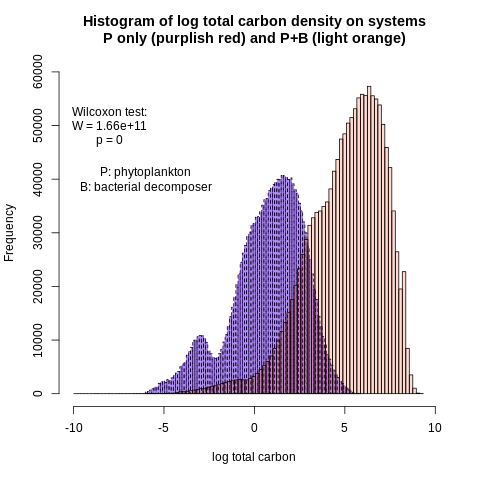
\includegraphics[width=.7\linewidth]{report/media/hist_PvsPB_A.png}
    \caption{Histogram of distribution on sustainable yield for total carbon in the system across the whole parameter space}
    \label{hist:A}
\end{figure}

Fig.\ref{hist:A} is the distribution of sustainable yield between the equilibrium position between phytoplankton only [P] and phytoplankton \& bacterial decomposer [P+B] set-ups.
\begin{itemize}
    \item both distributions are not normally-distributed $\rightarrow$ non-parametric test
    \item Wilcox-test: significantly different
    \item P+B $>$ P
\end{itemize}

Criticism: is the difference only due to the incorporation of bacterial biomass?
\begin{itemize}
    \item org-C: P+B $<$ P (Fig.\ref{hist:C})
    \item org-P: P+B == P (by eqm position calculation)
    \item org-B: P+B $>$ 0, P == 0 (by definition, P-only setting has no bacteria)
\end{itemize}
The figure not only indicated the effect by incorporating B, but also the reduction of org-C due to the carbon processing by B.  Yet the overall effect is still making P+B $>$ P in overall carbon in log-scale

\begin{figure}[H]
    \centering
    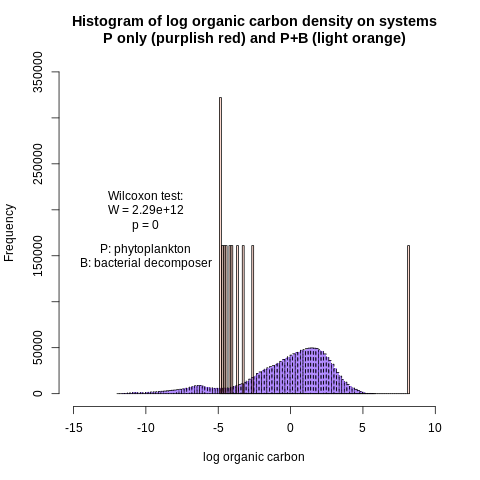
\includegraphics[width=.7\linewidth]{report/media/hist_PvsPB_C.png}
    \caption{Histogram of distribution on sustainable yield for organic carbon pool across the whole parameter space}
    \label{hist:C}
\end{figure}

Criticism: why do the distribution in ``total carbon" choppy?

\begin{figure}
    \centering
    \includegraphics[width=.7\linewidth]{}
    \caption{Plot of log organic carbon density against bacterial growth rate per unit organic carbon density ($\frac{m^3}{gC\cdot day}$)}
    \label{fig:orgCVSgB}
\end{figure}

\end{document}
